\section{The sum rule and the main theorem}\label{sec:sumrule}

\subsection{The sum rule}

\begin{theorem}\label{thm:sumrule}
Let $H=\sigma e^{ih}$ be a zero-free passive system that is regular on the
band, with phase $\varphi$, attenuation $\alpha$ and Herglotz measure $\mu$.
Then
\begin{equation}\label{eq:sumrule}
\int_a^b\alpha(\omega)\dd\omega
=\frac12\int_a^b\varphi(\omega)\,p(\omega)\dd\omega
+\frac\pi4\int_{\R\setminus S}W(t)\dd\mu(t),
\end{equation}
and every term is finite. The last integral is nonnegative, and it vanishes
if and only if $\mu(\R\setminus S)=0$.
\end{theorem}

The proof uses one fact about the Hilbert transform $\mathcal Hf(x)=\pi^{-1}
\PV\int f(t)\dd t/(x-t)$ on the line, the antisymmetry
\begin{equation}\label{eq:riesz}
\int_\R f\,\mathcal Hg\dd x=-\int_\R(\mathcal Hf)\,g\dd x ,
\qquad f\in L^{q},\ g\in L^{q'},
\end{equation}
valid for $1<q<\infty$ by M.~Riesz's theorem \cite{titchmarsh,king}.\footnote{Riesz's theorem is the boundedness of $\mathcal H$ on $L^q$, $1<q<\infty$. For smooth compactly supported $f,g$ the antisymmetry is Fubini's theorem for the truncated kernel $\mathbf 1_{\abs{x-t}>\varepsilon}/(x-t)$, which is odd under $x\leftrightarrow t$; it extends to $L^q\times L^{q'}$ by density and Riesz's bound.}

\begin{proof}
\emph{Finiteness.} $\varphi$ is continuous on $[a,b]$ and $p$ is integrable.
On $I\setminus[a,b]$ the measure is $\pi^{-1}\alpha\dd t$ with $\alpha$
bounded (\cref{lem:regular}), and $W$ has integrable singularities at
$a,b$. Away from $I\cup(-I)$, $W$ is bounded and $O(t^{-4})$, while
$\int\dd\mu/(1+t^2)<\infty$.

\emph{Decomposition.} Choose $a_1<a$ and $b_1>b$ with $[a_1,b_1]\subset I$,
let $I_1=(a_1,b_1)$, and split $\mu=\mu_1+\mu_2$ with $\mu_1$ the restriction
of $\mu$ to $I_1\cup(-I_1)$. By \eqref{eq:foster},
\begin{gather*}
h=\beta z+h_1+h_2,\\
h_j(z)=-\frac{\mu_j(\{0\})}{z}+\int_{(0,\infty)}\frac{2z}{t^2-z^2}\dd\mu_j(t),
\end{gather*}
and $\varphi=\beta x+\Re h_1+\Re h_2$ on $(a,b)$.

\emph{The delay.} $\frac12\int_a^b\beta x\,p(x)\dd x=0$ by
\cref{lem:moments}(i).

\emph{The far part.} The measure $\mu_2$ has no mass in $I_1\cup(-I_1)$, so
$h_2$ is continuous up to $(a,b)$ and the kernel $2x/(t^2-x^2)$ is bounded by
a constant times $(1+t^2)^{-1}$ for $x\in[a,b]$ and $t\notin I_1$. Fubini's
theorem and \cref{lem:kernel,lem:moments}(iii) give
\begin{align*}
\frac12\int_a^b\Re h_2\,p\dd x
&=-\frac{\mu(\{0\})}2\int_a^b\frac px\dd x-\frac\pi2\int_{(0,\infty)\setminus I_1}W\dd\mu\\
&=-\frac\pi4\int_{\R\setminus(I_1\cup-I_1)}W\dd\mu ,
\end{align*}
where we used $W(0)=(b-a)^2/(ab)$,\footnote{$\rho(0)=\sqrt{a/b}\sqrt{a/b}=a/b$, so $W(0)=a/b-2+b/a=(b-a)^2/(ab)$. With \cref{lem:moments}(iii), $\int_a^bp/x\dd x=\pi(b-a)^2/(2ab)=\frac\pi2W(0)$, which turns the atom at $0$ into $-\frac\pi4W(0)\mu(\{0\})$.} the evenness of $W$ on $\R\setminus S$
and of $\mu$.

\emph{The near part.} Here $\mu_1=\psi(t)\dd t$ with $\psi=\pi^{-1}\alpha(\abs
t)$ on $I_1\cup(-I_1)$, a bounded function. For almost every $x\in(a,b)$,
\begin{align*}
\Re h_1(x)&=\PV\int_{I_1}\psi(t)\frac{2x}{t^2-x^2}\dd t\\
&=\PV\int_{I_1}\psi(t)\Big(\frac1{t-x}-\frac1{t+x}\Big)\dd t ,
\end{align*}
the boundary value of the real part of a Cauchy integral with bounded
density \cite{king,muskhelishvili}. We claim that
\begin{multline}\label{eq:swap}
\int_a^bp(x)\,\Re h_1(x)\dd x\\
=\int_{I_1}\psi(t)\Big(\PV\int_a^bp(x)\frac{2x}{t^2-x^2}\dd x\Big)\dd t .
\end{multline}
For the part $1/(t+x)$ of the kernel this is Fubini's theorem, the kernel
being bounded. For the part $1/(t-x)$ it is \eqref{eq:riesz} with
$f=p\,\mathbf 1_{[a,b]}\in L^{3/2}$ and $g=\psi\mathbf 1_{I_1}\in L^{3}$; the
function $p$ lies in $L^q$ for every $q<2$ because its singularities are of
order $\abs{x-a}^{-1/2}$ and $\abs{x-b}^{-1/2}$. By \cref{lem:kernel}
the inner integral in \eqref{eq:swap} equals $2\pi$ for $t\in(a,b)$ and
$-\pi W(t)$ for $t\in I_1\setminus[a,b]$. Hence
\begin{align*}
\frac12\int_a^bp\,\Re h_1\dd x&=\pi\int_a^b\psi\dd t-\frac\pi2\int_{I_1\setminus[a,b]}W\dd\mu\\
&=\int_a^b\alpha\dd t-\frac\pi4\int_{(I_1\cup-I_1)\setminus S}W\dd\mu .
\end{align*}

Adding the three parts gives \eqref{eq:sumrule}. Since $W>0$ on $\R\setminus
S$ and $\mu$ has no atoms at $\pm a,\pm b$, the last term vanishes exactly
when $\mu(\R\setminus S)=0$.
\end{proof}

The identity \eqref{eq:sumrule} holds for every phase. Its content is that
the band loss is a fixed linear functional of the band phase plus a
nonnegative price for everything the system does outside the band: a
lossless resonance at $\omega_0\notin[a,b]$ with weight $\gamma$ in $\mu$ costs
$\frac\pi2W(\omega_0)\gamma$,\footnote{The measure is even, so the resonance puts mass $\gamma$ at both $\pm\omega_0$, and $W(-\omega_0)=W(\omega_0)$ off the band; the two atoms give $\frac\pi4\cdot2W(\omega_0)\gamma$.} a pole at the origin costs
$\frac\pi4W(0)\mu(\{0\})$, and absorption outside the band costs its
$W$-weighted total.

\subsection{Constant phase lag}

Put
\begin{equation}\label{eq:Lambda}
\begin{aligned}
\Lambda&=\frac{J}{2(b-a)}\\
&=\frac1{2(b-a)}\int_a^b
\frac{a^2+b^2-2\omega^2}{\sqrt{(\omega^2-a^2)(b^2-\omega^2)}}\dd\omega>0 .
\end{aligned}
\end{equation}
\Cref{sec:constant} shows $\Lambda=(K(\kappa)-E(\kappa))/\kappa$.

\begin{theorem}[Main theorem]\label{thm:main}
Let $H$ be a zero-free passive system, regular on the band $[a,b]$, whose
phase on the band is
\[
\varphi(\omega)=\theta+\tau\omega,\qquad a<\omega<b,
\]
with $\theta\ge0$ and $\tau\in\R$. Then
\begin{equation}\label{eq:main}
\frac1{b-a}\int_a^b\alpha(\omega)\dd\omega\ \ge\ \theta\,\Lambda .
\end{equation}
Equality holds if and only if $\mu(\R\setminus S)=0$; for every $\theta\ge0$
it is attained by the system $H_\star$ of \cref{thm:extremal}.
\end{theorem}

\begin{proof}
By \cref{lem:moments}(i),
$\frac12\int_a^b(\theta+\tau\omega)p\dd\omega=\frac12\theta J=(b-a)\theta\Lambda$,
and \cref{thm:sumrule} gives the inequality and the case of equality.
\end{proof}

Three remarks make the statement concrete.

\begin{remark}[Constant argument]\label{rem:arg}
If $\arg H\equiv\theta$ modulo $2\pi$ on the band, then
$\varphi=\theta-\frac{1-\sigma}2\pi$ modulo $2\pi$, and since $\varphi$ is
continuous it is a constant $\theta'$ with $\theta'\equiv\theta\pmod\pi$. The
theorem applies with $\theta'$ when $\theta'>0$. Which representative occurs
is not decided by the band: it depends on how much phase the system has
accumulated from the imaginary axis, for instance from zero frequency.
\end{remark}

\begin{remark}[Lossless resonances]\label{rem:resonances}
The equality case shows that every lossless resonance outside the band, and
every atom of $\mu$ at zero frequency, raises the loss strictly above the
bound. Shaping the phase with reactances, the classical tool of all-pass and
phase-equaliser design, therefore works against a constant phase lag.
\Cref{fig:cost} shows the price of a unit of measure off the band, the
factor $\frac\pi4W(t)$ of \eqref{eq:sumrule}.
\end{remark}

\begin{figure}[t]
\centering
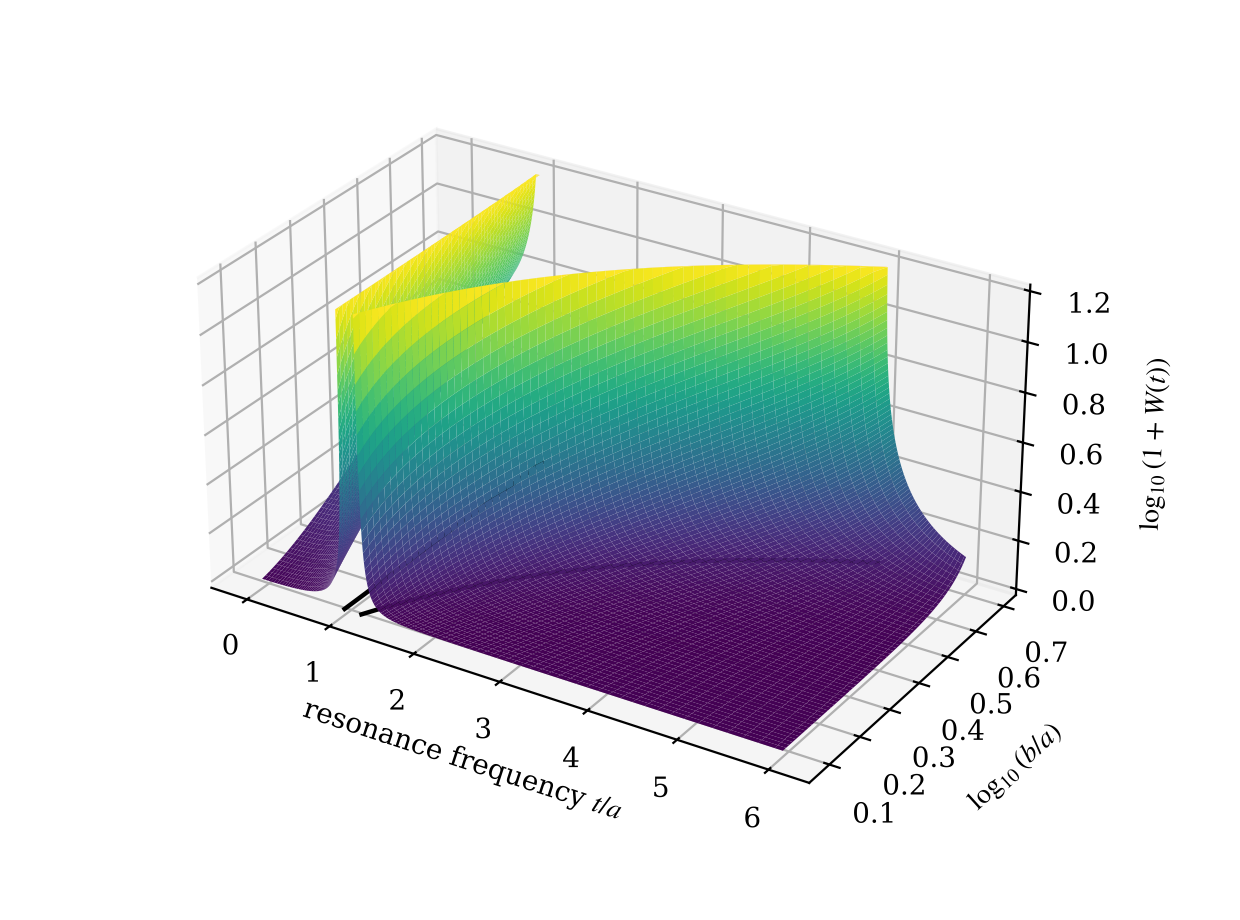
\includegraphics[width=\columnwidth]{figures/fig_cost.png}
\caption{The cost $\log_{10}(1+W(t))$ of a lossless resonance at frequency
$t$, as a function of $t/a$ and of the band ratio $b/a$. It vanishes only on
the band (the gap between the two sheets), grows without bound at the band
edges, and decays like $t^{-4}$ at high frequency (\cref{lem:W}(i)); at
$t=0$ it is $W(0)=a/b+b/a-2>0$.}
\label{fig:cost}
\end{figure}

\begin{remark}[Passivity everywhere is needed]\label{rem:cpe}
The constant-phase element $H(z)=(-iz/a)^{-\gamma}$, $0<\gamma<1$, familiar
from dielectric relaxation \cite{westerlund}, has phase $\theta=\gamma\pi/2$ at
every positive frequency and attenuation $\alpha=\gamma\log(\omega/a)\ge0$
on $[a,\infty)$. Over an octave its mean attenuation is
$(2\theta/\pi)(2\log2-1)=0.2459\,\theta$, below the bound
$0.2735\,\theta$. There is no contradiction: $\abs H>1$ for $\omega<a$, so $H$
is not passive. The bound depends on passivity at all frequencies, not only
on the band.
\end{remark}

\subsection{Constant phase lead}

For a negative intercept the same identity, applied after an inversion of
the frequency axis, gives a weighted bound.

\begin{theorem}\label{thm:lead}
Let $H$ be as in \cref{thm:main} but with $\theta<0$. Then
\begin{equation}\label{eq:lead}
\frac1{b-a}\int_a^b\alpha(\omega)\,\frac{ab}{\omega^2}\dd\omega
\ \ge\ \abs\theta\,\Lambda-\frac\pi4\,\tau\,(b-a).
\end{equation}
For $\tau=0$ equality holds if and only if $\beta=0$ and $\mu$ vanishes on
$\R\setminus(S\cup\{0\})$; it is attained by $H_\star(-ab/z)$, where $H_\star$
is the extremal system for $\abs\theta$.
\end{theorem}

\begin{proof}
The map $z\mapsto-ab/z$ preserves $\Cp$, so $\tilde h(z)=h(-ab/z)$ is a
Herglotz function with the symmetry of \eqref{eq:Hh}, and $\tilde H=\sigma
e^{i\tilde h}$ is zero-free, passive and regular on the band, since
$x\mapsto ab/x$ maps a neighbourhood of $[a,b]$ onto another. For $x\in(a,b)$
the point $-ab/(x+i0)$ lies above $-ab/x\in(-b,-a)$, so by the oddness of
$\varphi$,
\[
\tilde\varphi(x)=-\varphi(ab/x),\qquad\tilde\alpha(x)=\alpha(ab/x).
\]
Substituting $x=ab/\omega$ and using $r(ab/\omega)=ab\,r(\omega)/\omega^2$,
\begin{gather*}
\int_a^bf(ab/x)\,p(x)\dd x=\int_a^bf(\omega)\,p^*(\omega)\dd\omega,\\
p^*(\omega)=\frac{a^2+b^2-2a^2b^2/\omega^2}{r(\omega)},
\end{gather*}
for every integrable $f$. With $f=1$ and $f(\omega)=\omega$ this gives
$\int_a^bp^*=J$ and $\int_a^b\omega p^*=ab\int_a^bp/x=\pi(b-a)^2/2$
(\cref{lem:moments}(iii)). \Cref{thm:sumrule} for $\tilde H$ now reads
\[
\int_a^b\alpha(\omega)\frac{ab}{\omega^2}\dd\omega
=-\frac12\int_a^b(\theta+\tau\omega)p^*\dd\omega+\frac\pi4\int_{\R\setminus S}W\dd\tilde\mu ,
\]
which is \eqref{eq:lead} after division by $b-a$. The measure $\tilde\mu$
is the image of $\mu$ under $t\mapsto-ab/t$ with density $ab/t^2$ on
$\R\setminus\{0\}$, plus an atom $ab\beta$ at $0$ coming from the term
$\beta z$; an atom of $\mu$ at $0$ becomes a linear term of $\tilde h$ and
costs nothing. This gives the case of equality, and $H_\star(-ab/z)$ has
$\beta=0$ and its measure on $S\cup\{0\}$.
\end{proof}

\subsection{The worst frequency}

\begin{corollary}\label{cor:worst}
Let $H$ be zero-free, passive and regular on the band, with $\arg
H\equiv\theta$ modulo $2\pi$ on $[a,b]$. Then
\[
\max_{[a,b]}\alpha\ \ge\ \dist(\theta,\pi\Z)\,\Lambda ,
\]
so at some frequency of the band the transmitted power is at most
$e^{-2\dist(\theta,\pi\Z)\Lambda}$. If the phase $\theta'$ of
\cref{rem:arg} is positive, also
\[
\exp\Big(\frac1{b-a}\int_a^b\log\abs{H(\omega)}^2\dd\omega\Big)\le e^{-2\theta'\Lambda},
\]
that is, the geometric mean of the power transmission over the band is at
most $e^{-2\theta'\Lambda}$.
\end{corollary}

\begin{proof}
By \cref{rem:arg} the phase is a constant $\theta'\equiv\theta\pmod\pi$. If
$\theta'>0$ then $\theta'\ge\dist(\theta,\pi\Z)$ and \cref{thm:main} bounds
the mean, hence the maximum, of $\alpha$. If $\theta'<0$ then
$\abs{\theta'}\ge\dist(\theta,\pi\Z)$, and since
$\int_a^bab\,\omega^{-2}\dd\omega=b-a$ the left side of \eqref{eq:lead}
with $\tau=0$ is at most $\max\alpha$. The
second statement is \eqref{eq:main} with $\log\abs H=-\alpha$.
\end{proof}

\begin{remark}[The lead extremal]\label{rem:leadmean}
For the system $H_\star(-ab/z)$ of \cref{thm:lead}, whose phase is
$-\abs\theta$ on the band, \cref{thm:sumrule} applied directly gives the
plain mean attenuation
\[
\frac1{b-a}\int_a^b\alpha\dd\omega
=\abs\theta\,\frac{E(\kappa)-\kappa'^2K(\kappa)}{\kappa},\qquad\kappa'^2=1-\kappa^2,
\]
because its measure off $S$ is the atom $ab\,\tau_\star$ at $0$, of cost
$\frac\pi4W(0)ab\tau_\star$, with $\tau_\star$ from \cref{thm:extremal} and the
evaluation of \cref{sec:constant}. For an octave this is $0.2656\abs\theta$,
slightly below $\Lambda=0.2735$. Whether it is the least plain mean among
systems with constant phase lead is not known.
\end{remark}
